%%%%%%%%%%%%%%%%%%%%%%%%%%%%%%%%%%%%%%%%%
% Simple Sectioned Essay Template
% LaTeX Template
%
% This template has been downloaded from:
% http://www.latextemplates.com
%
% Note:
% The \lipsum[#] commands throughout this template generate dummy text
% to fill the template out. These commands should all be removed when 
% writing essay content.
%
%%%%%%%%%%%%%%%%%%%%%%%%%%%%%%%%%%%%%%%%%

%----------------------------------------------------------------------------------------
%	PACKAGES AND OTHER DOCUMENT CONFIGURATIONS
%----------------------------------------------------------------------------------------

\documentclass[12pt]{article} % Default font size is 12pt, it can be changed here

\usepackage{geometry} % Required to change the page size to A4
\geometry{a4paper} % Set the page size to be A4 as opposed to the default US Letter

\usepackage{graphicx} % Required for including pictures

\usepackage{float} % Allows putting an [H] in \begin{figure} to specify the exact location of the figure
\usepackage{wrapfig} % Allows in-line images such as the example fish picture
\usepackage{multirow}

\usepackage{lipsum} % Used for inserting dummy 'Lorem ipsum' text into the template

\linespread{1.2} % Line spacing


%\setlength\parindent{0pt} % Uncomment to remove all indentation from paragraphs

\graphicspath{{Pictures/}} % Specifies the directory where pictures are stored

\begin{document}

%----------------------------------------------------------------------------------------
%	TITLE PAGE
%----------------------------------------------------------------------------------------

\begin{titlepage}

\newcommand{\HRule}{\rule{\linewidth}{0.5mm}} % Defines a new command for the horizontal lines, change thickness here


\center % Center everything on the page

\textsc{\LARGE   }\\[1.5cm] % Name of your university/college
\textsc{\Large No Other But a Woman's Reason}\\[0.5cm] % Major heading such as course name
\textsc{\large Textual Analysis of Gender in Shakespeare}\\[0.5cm] % Minor heading such as course title

\HRule \\[0.4cm]
%{ \huge \bfseries Title}\\[0.4cm] % Title of your document
%\HRule \\[1.5cm]

\begin{minipage}{0.4\textwidth}
\begin{flushleft} \large
\emph{Author:}\\
Katherine \textsc{Roe} % Your name
\end{flushleft}
\end{minipage}
~
\begin{minipage}{0.4\textwidth}
\begin{flushright} \large
\emph{Supervisor:} \\
Prof. Bob \textsc{Berwick} % Supervisor's Name
\end{flushright}
\end{minipage}\\[4cm]

{\large
}\large May 2015 % Date, change the \ to a set date if you want to be precise

%\includegraphics{Logo}\\[1cm] % Include a department/university logo - this will require the graphicx package

\vfill % Fill the rest of the page with whitespace

\end{titlepage}

%----------------------------------------------------------------------------------------
%	TABLE OF CONTENTS
%----------------------------------------------------------------------------------------

\tableofcontents % Include a table of contents

\newpage % Begins the essay on a new page instead of on the same page as the table of contents 

%----------------------------------------------------------------------------------------
%	INTRODUCTION
%----------------------------------------------------------------------------------------

\section{Introduction} % Major section

	William Shakespeare, widely regarded as one of the best playwrights in any language, created hundreds of well-known and timeless characters of both genders. Although many thousands of books and papers have examined the role of gender in Shakespeare’s plays, very few if any have performed a rigorous quantitative analysis of the texts. For my 6.UAP project, I have performed such an analysis on the lines delivered by men versus the lines delivered by women to determine whether Shakespeare wrote male and female characters in a quantifiably distinct manner. I analyzed the number of unique words, types of speech, sentence length, line length, and sentiment of every line in 36 Shakespeare plays. My aim in this project was to write text analysis software that can be used to shed light on subtle aspects of gender treatment in Shakespearean theater and other literature.

%----------------------------------------------------------------------------------------
%	MAJOR SECTION 1
%----------------------------------------------------------------------------------------

\section{Methods} % Major section


%------------------------------------------------

\subsection{Text} % Sub-section

	The first challenge was to represent Shakespeare’s plays in a way that allowed for data analysis. I started with an HTML version of every play analyzed. I then wrote a script that converted each line into a python object. These objects included the line’s play, location in the play, location in the speech, act and scene, speaker, speaker gender, and text.
%------------------------------------------------

\subsection{Analysis}
Once the plays were prepared, I wrote a series of Python scripts to analyze the texts along several dimensions. These dimensions were number of words per line, sentence length, speech length, lines delivered, and number of unique words. Additionally, I used natural language processing Python packages to analyze the parts of speech distribution, subjectivity, and polarity of each line.

\subsection{A Note on Categorization}
For the data analysis, I divided Shakespeare's  plays into comedies, histories, and tragedies as shown in Table 1.

\begin{center}
\begin{table}
\centering

\begin{tabular}{|l|l|l|}
  \hline
 \textsc{Comedies} & \textsc{Tragedies} & \textsc{Histories}\\
  \hline
  All's Well That Ends Well &  Antony and Cleopatra \hspace{8 mm} & King John \hspace{17 mm} \\

  As You Like It & Coriolanus & Richard II\\

  Comedy of Errors & Hamlet & Henry IV Part 1\\

  Cymbeline & Julius Caesar & Henry V\\

  Love's Labours Lost & King Lear & Henry VI Part 1\\

  Measure for Measure & Macbeth & Henry VI Part 2\\

  The Merchant of Venice & Othello & Henry VI Part 3\\

  The Merry Wives of Windsor & Romeo and Juliet & Richard III \\

  A Midsummer Night's Dream & Timon of Athens & Henry VIII \\

  Much Ado About Nothing & Titus Andronicus & \\

  Pericles &  & \\
  
  The Taming of the Shrew & & \\

 The Tempest & & \\

  Troilus and Cressida & & \\
  
  Twelfth Night & & \\
  
  Two Gentlemen of Verona & & \\
  
  The Winter's Tale & & \\
  \hline
\end{tabular}
	\caption{Shakespeare Play Categorization}
\end{table}
\end{center}


	

%----------------------------------------------------------------------------------------
%	MAJOR SECTION X - TEMPLATE - UNCOMMENT AND FILL IN
%----------------------------------------------------------------------------------------

\section{Results}

\subsection{Numerical Metrics}
Several strictly numerical metrics were used in the play analysis. These were number of lines, words per line, speech length, sentence length, and number of unique words spoken by men versus women in Shakespeare's plays.


\subsubsection{Total Lines}
An initial, obvious measure of gender differences can be found by counting the number of lines (here defined as a 10-syllable iambic pentameter unit) delivered by men and women in each play. Women were found to deliver strikingly fewer lines than their male counterparts, speaking just under 18\% of the total lines in all of the plays.  Even in The Merry Wives of Windsor, the eponymous wives deliver only 25\% of that play's lines, and the shrew delivers a meager 219 compared to her tamer's 586. The plays overall ranged from the relatively egalitarian As You Like It (37\% of lines delivered by women) to the incredibly masculine Timon of Athens (.4\% of lines delivered by women).

It is worth noting that the proportion of lines delivered by women varied drastically by play type. Women were fairly well represented in the comedies, enjoying 23\% of the total lines across the play type. In the tragedies, however, only 16\% of lines were spoken by women, and in the histories women spoke a paltry 12\% of lines. Figures 1, 2, and 3 show the number of lines spoken by gender for each of the plays, separated by play type.

\begin{figure}[H] % Example image
\center{\includegraphics[width=1.0\linewidth]{comedies_line_numbers}}
\caption{Total Lines in Shakespeare's Comedies}
\label{fig:speciation}
\end{figure}

\begin{figure}[H] % Example image
\center{\includegraphics[width=1.0\linewidth]{tragedies_line_numbers}}
\caption{Total Lines in Shakespeare's Tragedies}
\label{fig:speciation}
\end{figure}

\begin{figure}[H] % Example image
\center{\includegraphics[width=1.0\linewidth]{histories_line_numbers}}
\caption{Total Lines in Shakespeare's Histories}
\label{fig:speciation}
\end{figure}


\subsubsection{Words Per Line} % Sub-section
Shakespeare is well known for writing in iambic pentameter, meaning that, with very few exceptions, each line of his plays include ten syllables. Counting the average number of words per line, therefore, is a good measure for the average length of a spoken word. I postulated that female characters might have a higher number of average words per line, correlating to shorter words. Contrary to this expectation, men and women speak almost exactly the same number of words per line. In fact, in all the plays, men speak about 7.53 words per line compared to women's 7.41 (about a 1.6\% difference). Women consistently spoke fewer words per line than men in all three categories of play, although there were individual plays (such as Coriolanus) where the overall trend was reversed. The average number of words per line for men and women in the tragedies are shown in Figure 4.

\begin{figure}[H] % Example image
\center{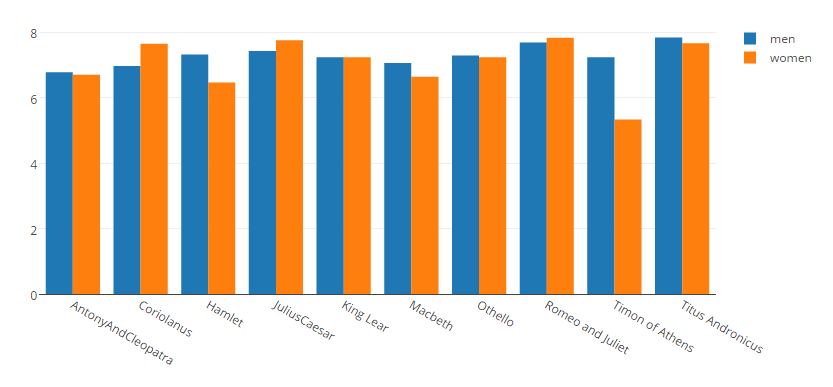
\includegraphics[width=1.0\linewidth]{wpl}}
\caption{Words per Line in Shakespeare's Tragedies}
\label{fig:speciation}
\end{figure}

\subsubsection{Sentence Length}
Another numerical measure was sentence length. I measured the average number of words per sentence spoken by men and women in all of the plays. Longer sentences suggest more complex thoughts, so I postulated that men would speak in slightly longer sentences than women. Although men did speak in slightly longer sentences, on average, than women, the difference was small. Men had an average sentence length of 13.125 words across all plays, compared to women's average sentence length of 12.833 words across all plays. Words per sentence for the comedies is shown in Figure 5.

\begin{figure}[H] % Example image
\center{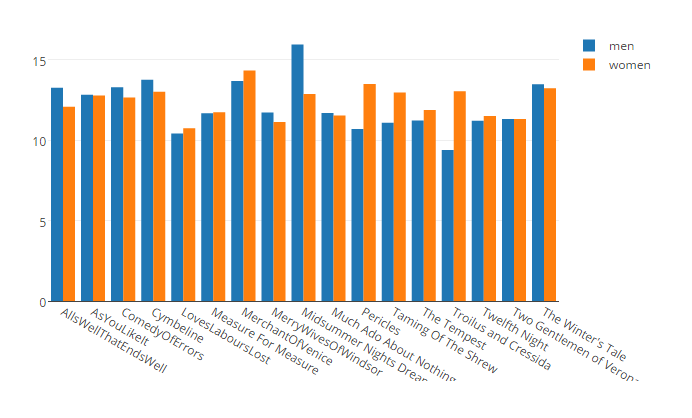
\includegraphics[width=1.0\linewidth]{sentencelength}}
\caption{Words per Sentence in Shakespeare's Comedies}
\label{fig:speciation}
\end{figure}

% Content

%------------------------------------------------



\subsubsection{Speech Length} % Sub-section
A measure related to sentence length is speech length. This simply measures how long each character speaks before another character interjects. I predicted that the speech length would be substantially longer for male characters than for their female counterparts. In fact, the average speech length was almost the same for men and women on average, at 26.2 words per speech for men and 26.4 words per speech for women. It is worth noting, however, that there was an enormous range for average speech length in different plays. For instance, women in Henry V have an average speech length of 7.4 words (compared to men's 39.5), whereas women in Julius Caesar enjoy an average speech length of 47.1 words (compared to men's 24.5). The data for all plays are shown in Figure 6.

\begin{figure}[H] % Example image
\center{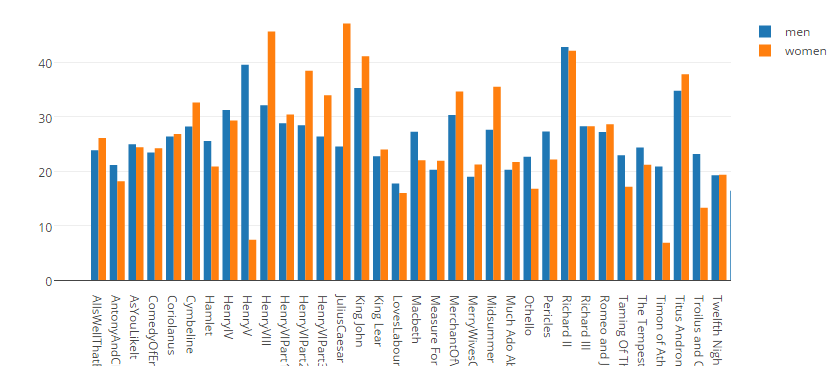
\includegraphics[width=1.0\linewidth]{speechlength}}
\caption{Words per Speech in Shakespeare's Plays}
\label{fig:speciation}
\end{figure}

The data may have been slightly skewed by minor characters, such as unnamed servants and nobles, who are almost invariably male and tend to have shorter speeches. Closer analysis of major characters may reveal a different distribution. Furthermore, there are so few female characters in many of the plays that the data is perhaps not statistically significant. For instance, in Henry V, only 150 of the play's 3403 lines (10-syllable blank verse lines, not speeches) are delivered by women. The small proportion of lines delivered by women accounts for the variance seen in female line length.

\subsubsection{Unique Words}
Another measurement of thought complexity is the number of unique words used in speech. I didn't expect this measure to vary significantly between men and women, and this prediction largely proved correct. Although men do use more unique words than women (30486 across all plays compared to 12883 spoken by women), this is most likely a reflection of the substantially larger number of lines spoken by men. Indeed, when I compared the same amount of text spoken by men and women across the plays, I found that men used 1613 unique words compared to women's 1572 words over 5000 lines. This represents a difference of just 2.6\% between the genders.

\subsection{Natural Language Processing}
In addition to the numerical metrics, several measurements were made with the Natural Language Toolkit and TextBlob for Python. These measurements include parts of speech distribution, subjectivity, and polarity.


\subsubsection{Parts of Speech}
One measure of speaking style is determining the breakdown of parts of speech. Table 2 outlines the findings for POS breakdown for men and women. The "Other" category includes a wide range of uncommon types, including foreign words, numbers, and the word "to".

Although the differences in parts of speech are slight between men and women, they are statistically significant in several cases. Particularly notable is the fact that pronouns are 7\% more common in female speech than in male speech. A possibly hypothesis for this discrepancy is that women are more likely to be talking about other characters than about objects and places. This hypothesis is supported by the fact that the most common pronouns are almost all third person male pronouns. However, further analysis into the types of pronouns spoken by men and women is required before a definitive conclusion can be reached.

\begin{center}
\begin{table}
\centering

\begin{tabular}{|l|l|l|}
  \hline
 \textsc{POS} & \textsc{Men} & \textsc{Women}\\
  \hline
  Nouns & 23.8\% & 23.0\% \\
  Verbs & 15.9\% & 16.3\% \\
  Pronouns & 19.8\% & 21.2\% \\
  Adjectives & 6.9\% & 7.0\% \\
  Adverbs & 5.4\% & 5.7\% \\
  Prepositions & 10.4\% & 10.0\% \\
  Coord. Conjunctions & 4.0\% & 3.8\% \\
  Determiners & 7.7\% & 7.0\% \\
  Possessive Endings & 2.9\% & 3.0\% \\
  Other & 3.2\% & 3\%\\
  \hline
\end{tabular}
	\caption{Parts of Speech by Gender}
\end{table}
\end{center}

\subsubsection{Subjectivity}
Subjectivity and the following metric, polarity, were measured using the sentiment analysis on TextBlob for Python. A naive Bayes analyzer trained on movie reviews determines the subjectivity from 0.0 (very objective) to 1.0 (very subjective). Although there is a fairly high error rate for this type of analysis, it nevertheless can be useful for discerning broader trends in the data.

The data did, in fact, reveal a correlation between gender and subjectivity. The average female line scored a .254, which is 10.4\% more subjective than the average male line's score of .230. This trend held throughout the comedies, tragedies, and histories, although there were individual plays, such as The Taming of the Shrew, which bucked the trend. The data for the comedies is presented in Figure 7.

\begin{figure}[H] % Example image
\center{\includegraphics[width=1.0\linewidth]{comedy_subjectivity}}
\caption{Line Subjectivity in the Comedies}
\label{fig:speciation}
\end{figure}

It is worth noting, as was observed previously, that almost every minor character is male in Shakespeare's plays. Analyzing only the subjectivity of main characters could render male and female characters approximately equally subjective, as minor characters are intuitively more likely to report facts and events than to declare strong feelings.

\subsubsection{Polarity}
Line polarity was measured through the same sentiment analysis tool as the subjectivity. Polarity measures how positive, negative, or neutral a line is, and ranges from -1 to 1. A score of 0 indicates a perfectly neutral text.

Female lines were found to have more polar lines in either direction, and also to be more positive than male characters on average. The average female line had a polarity with an absolute value of .153, whereas the average male line has a polarity with an absolute value of .141. These numbers indicate that female lines were approximately 8.5\% more polar than male lines.

When the net value was considered (allowing positive and negative lines to cancel each other), the average female polarity was .077 compared to the average male polarity of .053. These differences indicate that women in Shakespeare are more likely to express strong emotions in any particular line, and that they are also slightly more positive on average than their male counterparts.

The average absolute and net polarities are shown in Figures 8 and 9, respectively.

\begin{figure}[H] % Example image
\center{\includegraphics[width=1.0\linewidth]{absolute_polarity}}
\caption{Absolute Line Polarity in the Comedies}
\label{fig:speciation}
\end{figure}

\begin{figure}[H] % Example image
\center{\includegraphics[width=1.0\linewidth]{net_polarity}}
\caption{Net Line Polarity in the Comedies}
\label{fig:speciation}
\end{figure}
% Content

%----------------------------------------------------------------------------------------
%	CONCLUSION
%----------------------------------------------------------------------------------------

\section{Conclusion} % Major section

In conclusion, initial analysis suggested that women and men speak similarly in Shakespeare's plays, although men speak far more. Women and men use similar word lengths, sentence lengths, and speech lengths, and share a similarly rich vocabulary. Using language analysis tools, however, certain differences can be uncovered. Women, for instance, are more likely to use certain parts of speech, such as pronouns, than their male counterparts. This may suggest that women are more likely to talk about other characters, particularly given that the plurality of pronouns are third person male pronouns.

Additionally, female lines tend to be substantially more subjective and polar than male lines. This difference suggests that Shakespeare wrote female characters, on average, as less logical and more emotional than male characters, echoing the prevailing notions on gender differences in Elizabethan England.

%----------------------------------------------------------------------------------------
%	BIBLIOGRAPHY
%----------------------------------------------------------------------------------------

\section{Acknowledgments} % Major section

For the parts of speech and sentiment analysis I used TextBlob, built on pattern and NLTK for Python. Graphs were made using Plotly, a graphing library for Python. Additionally, I would like to thank to Professor Bob Berwick for his invaluable guidance in this project.

%----------------------------------------------------------------------------------------

\end{document}